\documentclass[a4paper]{article}
\usepackage[portuguese]{babel}
\usepackage[utf8]{inputenc}
\usepackage{listings}
\usepackage{graphicx}
\usepackage{float}

\lstset{
numbers=left,
numberstyle=\small,
numbersep=8pt,
language=R,
breaklines=true,
tabsize=4}

\title{Exercício 8 - KNN}

\author{Reconhecimento de Padrões - UFMG}

\date{\small{Guilherme Capanema de Barros (\today)}}

\begin{document}
\maketitle

\section{Introdução}

O KNN (\textit{K nearest neighbours}) é um método de classificação determinístico que calcula a distância entre um ponto no espaço e os seus K vizinhos mais próximos.

O algoritmo pode ser implementado de diversas formas. Neste trabalho, a métrica de distância utilizada foi a \textbf{distância euclidiana}, e a classificação foi do tipo \textbf{maioria simples}: se a maioria dos K vizinhos mais próximos de um ponto for de uma determinada classe, o ponto pertencerá a essa classe.

\section{Implementação}

O KNN foi implementado na função abaixo. Ela recebe uma amostra a ser classificada, todos os dados de treinamento, os rótulos dos dados de treinamento e o parâmetro $K$.

\lstinputlisting{../myKNN.R}

\section{Experimentos}

O ajuste do parâmetro $K$ pode gerar uma classificação adequada, \textit{underfitting} (se $K$ for muito alto) ou \textit{overfitting} (se $K$ for muito baixo).

\subsection{Underfitting}

Para demonstrar uma situação de \textit{underfitting}, foi gerada uma base de dados sintética em espiral. O parâmetro definido foi $K = 20$. Os resultados estão exibidos na Fig. \ref{fig:underfitting}

\begin{figure}[H]
	\centering
	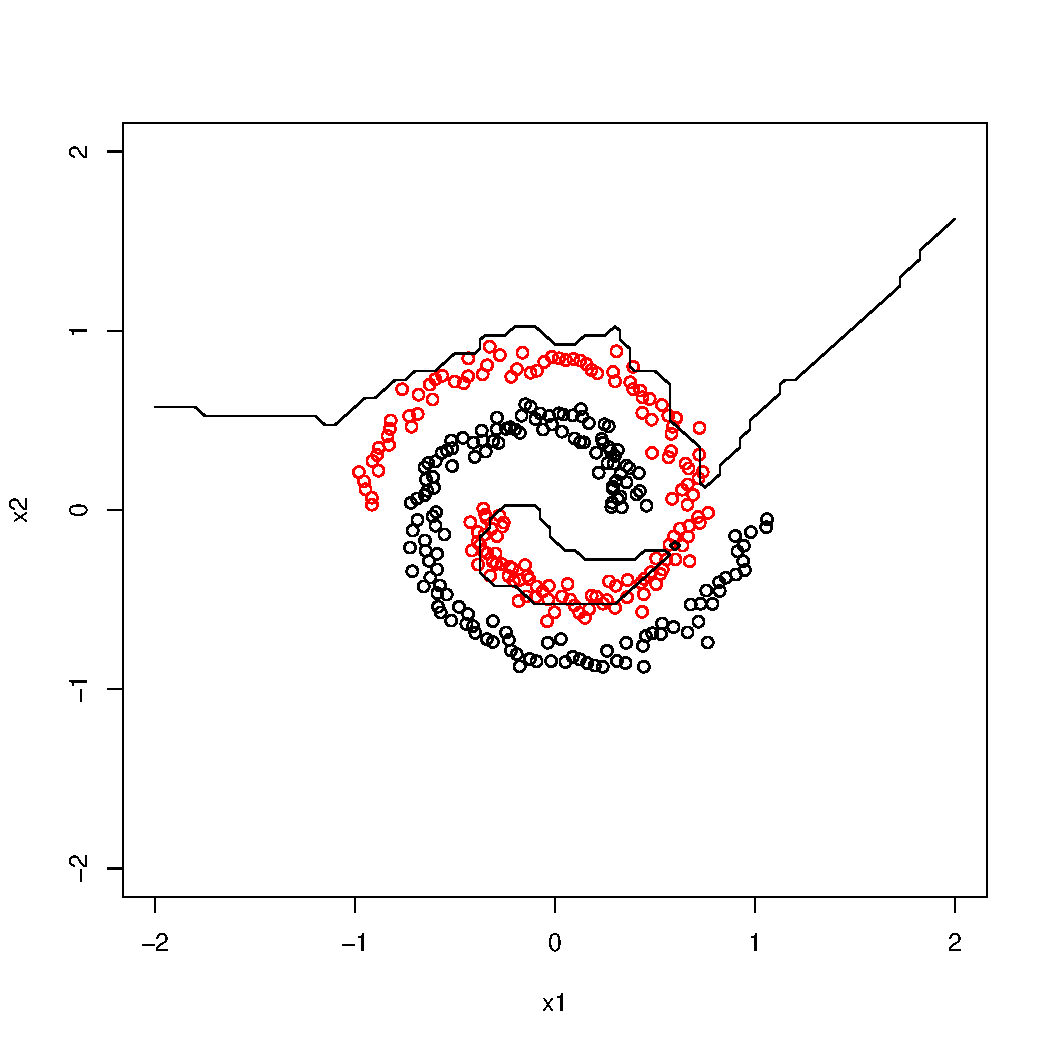
\includegraphics[page=1,width=0.7\textwidth]{../underfitting.pdf}
	\caption{\textit{Underfitting} para $K = 20$}
	\label{fig:underfitting}
\end{figure}

Abaixo, o código usado para gerar essa visualização:

\lstinputlisting{../underfitting.R}

\subsection{Overfitting}

Para demonstrar uma situação de \textit{overfitting}, foi gerada uma base de dados sintética de duas classes. O parâmetro definido foi $K = 2$. Os resultados estão exibidos na Fig. \ref{fig:overfitting}

\begin{figure}[H]
	\centering
	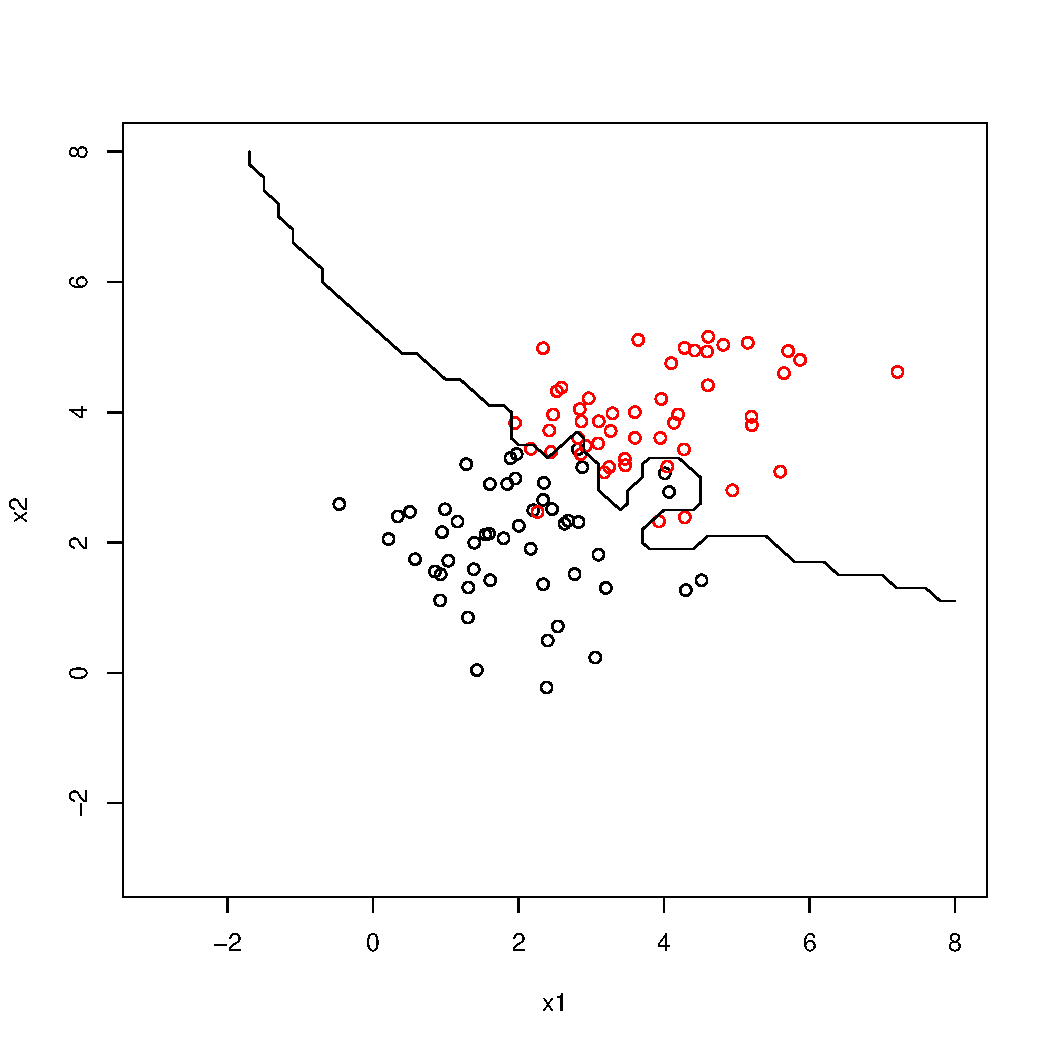
\includegraphics[page=1,width=0.7\textwidth]{../overfitting.pdf}
	\caption{\textit{Overfitting} para $K = 2$}
	\label{fig:overfitting}
\end{figure}

Abaixo, o código usado para gerar essa visualização:

\lstinputlisting{../overfitting.R}

\section{Conclusão}

Apesar da simplicidade, o KNN demonstra resultados razoáveis nas bases de dados testadas. O ajuste de $K$ pode ser feito, por exemplo, usando a validação cruzada \textit{10-fold}.

Para bases de dados desbalanceadas, é necessário cuidado no ajuste de $K$.

\end{document}
